\section{Evaluation Scheme}
The metric used in the competition for evaluating the models is accuracy. Additionally, we assess the model using precision, recall and F1-score in our work. We define them formally in the following subsection.

\subsection{Definitions}
% \sdaltcomment{Is this section required??}
% \sdaltcomment{Prec/Rec are only for label 1...}
We use the following notations in the definition of the metrics.
\begin{itemize}
    \item \textbf{TP} (True Positive): Model predicts hate spreader and is actually hate spreader.
    \item \textbf{FP} (False Positive): Model predicts hate spreader but is actually not hate spreader.
    \item \textbf{FN} (False Negative): Model predicts not hate spreader but is actually hate spreader.
    \item \textbf{TN} (True Negative): Model predicts not hate spreader and is actually not hate spreader.
\end{itemize}

The metrics mentioned earlier can be defined as follows:
\begin{table}[htpb]
\centering
\begin{tabular}{lcl}
Accuracy & = & $\frac{TP + TN}{TP + FP + FN + TN}$ \\
~ & ~ & ~ \\
Precision & = & $\frac{TP}{TP + FP}$ \\
~ & ~ & ~ \\
Recall & = & $\frac{TP}{TP + FN}$ \\
~ & ~ & ~ \\
F1-score & = & $\frac{2 \times \text{Precision} \times
\text{Recall}}{\text{Precision}+\text{Recall}}$ \\
\end{tabular}
\end{table}

\section{Baselines}

\subsection{Term-frequency based representation}
\label{sec:results:tf-idf}

% Please add the following required packages to your document preamble:
% \usepackage{multirow}
\begin{table}[htpb]
\centering
\begin{tabular}{llrrrr}
\hline
\textbf{Representation} & \textbf{Classifier} & \multicolumn{1}{l}{\textbf{Accuracy}} & \multicolumn{1}{l}{\textbf{Precision}} & \multicolumn{1}{l}{\textbf{Recall}} & \multicolumn{1}{l}{\textbf{F1-score}} \\ \hline
\multirow{4}{*}{Count} & LR & 0.6500 & 0.6531 & 0.6400 & 0.6465 \\ 
 & SVM & 0.6600 & 0.6600 & 0.6600 & 0.6600 \\ 
 & NB & 0.6200 & 0.6111 & 0.6600 & 0.6346 \\ 
 & RF & 0.6500 & 0.6596 & 0.6200 & 0.6392 \\ \hline
\multirow{6}{*}{TF-IDF} & LR & \textbf{0.6900} & 0.6792 & 0.7200 & 0.6990 \\ 
 & SVM & \textbf{0.6900} & 0.6667 & 0.7600 & 0.7103 \\ 
 & NB & 0.6600 & 0.6026 & 0.9400 & {0.7344} \\ 
 & RF & 0.6100 & 0.6000 & 0.6600 & 0.6286 \\ 
 & XGB & 0.6000 & 0.6136 & 0.5400 & 0.5745 \\ 
 & LGBM & 0.6200 & 0.6034 & 0.7000 & 0.6481 \\ \hline
\end{tabular}
\caption{Performance of models trained with Term-frequency based representation (Section \ref{sec:models:tf-idf})}
\label{tab:results:performance-tf-based}
\end{table}
% \sdaltcomment{use acro in tables?}

From Table \ref{tab:results:performance-tf-based}, it can be observed that both \ac{TF-IDF}+\ac{LR} and \ac{TF-IDF}+\ac{SVM} have the best performance in terms of accuracy (69\%). However, \ac{TF-IDF}+\ac{NB} has the highest F1-score (73.43\%) among all the models. It also has a very high recall score of 94\%, i.e., it produces the least low false negatives. \ac{TF-IDF}+\ac{SVM} also has a competitive F1-score score of 71.02\%. Moreover, \ac{TF-IDF} vectorization performs better than simple Count vectorization. The best hyper-parameter values obtained after fine-tuning are listed in Table \ref{tab:best-hparams-tf-based-count-vect} (with Count Vectorizer) and Table \ref{tab:best-hparams-tf-based-tfidf-vect} (with \ac{TF-IDF} Vectorizer).


% % Please add the following required packages to your document preamble:
% % \usepackage{multirow}
% \begin{table}[htbp]
% \centering
% \begin{tabular}{llr}
% \hline
% \textbf{Model} & \textbf{Hyper-parameter} & \textbf{Values} \\ \hline
% \multirow{8}{*}{LR} & (Vectorizer) &  \\
%  & max\_df & 0.75 \\
%  & min\_df & 2 \\
%  & ngram\_range & (1, 2) \\
%  & (Classifier) &  \\
%  & C & 2 \\
%  & penalty & l1 \\
%  & solver & saga \\  \hline
% \multirow{7}{*}{SVM} & (Vectorizer) &  \\
%  & max\_df & 0.75 \\
%  & min\_df & 2 \\
%  & ngram\_range & (1, 2) \\
%  & (Classifier) &  \\
%  & C & 0.1 \\
%  & kernel & linear \\  \hline
% \multirow{6}{*}{NB} & (Vectorizer) &  \\
%  & max\_df & 1.0 \\
%  & min\_df & 2 \\
%  & ngram\_range & (1, 1) \\
%  & (Classifier) &  \\
%  & alpha & 0.005623413251903491 \\  \hline
% \multirow{11}{*}{RF} & (Vectorizer) &  \\
%  & max\_df & 1.0 \\
%  & min\_df & 5 \\
%  & ngram\_range & (1, 2) \\
%  & (Classifier) &  \\
%  & bootstrap & True \\
%  & max\_depth & 10 \\
%  & max\_features & auto \\
%  & min\_samples\_leaf & 2 \\
%  & n\_estimators & 100 \\
%  & oob\_score & True \\  \hline
% \end{tabular}
% \caption{Best hyper-parameter values for models trained with Term-frequency based representation (Section \ref{sec:models:tf-idf}) with Count Vectorizer \sdaltcomment{too long.. take transpose... move to Appendix?} }
% \label{tab:best-hparams-tf-based-count-vect}
% \end{table}

% % Please add the following required packages to your document preamble:
% % \usepackage{multirow}
% % \usepackage{longtable}
% % Note: It may be necessary to compile the document several times to get a multi-page table to line up properly
% \begin{longtable}[c]{llr}
% \hline
% \textbf{Model} & \textbf{Hyper-parameter} & \textbf{Values} \\ \hline
% \endhead
% %
% \multirow{8}{*}{LR} & (Vectorizer) &  \\
%  & max\_df & 1.0 \\
%  & min\_df & 10 \\
%  & ngram\_range & (1, 1) \\
%  & (Classifier) &  \\
%  & C & 10 \\
%  & penalty & l2 \\
%  & solver & saga \\ \hline
% \multirow{7}{*}{SVM} & (Vectorizer) &  \\
%  & max\_df & 0.75 \\
%  & min\_df & 10 \\
%  & ngram\_range & (1, 1) \\
%  & (Classifier) &  \\
%  & C & 2 \\
%  & kernel & rbf \\ \hline
% \multirow{6}{*}{NB} & (Vectorizer) &  \\
%  & max\_df & 0.75 \\
%  & min\_df & 10 \\
%  & ngram\_range & (1, 1) \\
%  & (Classifier) &  \\
%  & alpha & 3.1622776601683795 \\ \hline
% \multirow{11}{*}{RF} & (Vectorizer) &  \\
%  & max\_df & 0.75 \\
%  & min\_df & 5 \\
%  & ngram\_range & (1, 1) \\
%  & (Classifier) &  \\
%  & bootstrap & True \\
%  & max\_depth & None \\
%  & max\_features & auto \\
%  & min\_samples\_leaf & 1 \\
%  & n\_estimators & 200 \\
%  & oob\_score & True \\ \hline
% \multirow{10}{*}{XGB} & (Vectorizer) &  \\
%  & max\_df & 1.0 \\
%  & min\_df & 2 \\
%  & ngram\_range & (1, 2) \\
%  & (Classifier) &  \\
%  & colsample\_bytree & 0.6 \\
%  & eta & 0.05 \\
%  & max\_depth & 7 \\
%  & n\_estimators & 100 \\
%  & subsample & 0.8 \\ \hline
% \multirow{10}{*}{LGBM} & (Vectorizer) &  \\
%  & max\_df & 1.0 \\
%  & min\_df & 10 \\
%  & ngram\_range & (1, 1) \\
%  & (Classifier) &  \\
%  & boosting\_type & dart \\
%  & colsample\_bytree & 0.6 \\
%  & learning\_rate & 0.05 \\
%  & n\_estimators & 50 \\
%  & subsample & 0.6 \\ \hline
% \caption{Best hyper-parameter values for models trained with Term-frequency based representation (Section \ref{sec:models:tf-idf}) with \ac{TF-IDF} Vectorizer \sdaltcomment{fix alignment...} }
% \label{tab:best-hparams-tf-based-tfidf-vect}\\
% \end{longtable}



%%%%%%%%%%%%%%%%%%%% SET UP 1 %%%%%%%%%%%%%%%%%%%
\begin{landscape}
\vspace*{\fill}
% Please add the following required packages to your document preamble:
% \usepackage{multirow}
\begin{table}[htbp]
    \centering
    \begin{tabular}{|l|rrr|rrrrrr|}
    \hline
    \multirow{2}{*}{\textbf{Model}} & \multicolumn{9}{c|}{\textbf{Hyper-parameters/Values}} \\
    \cline{2-10}
    & \multicolumn{3}{c|}{\textbf{Vectorizer}} & \multicolumn{6}{c|}{\textbf{Classifier}} \\
    \hline
    \multirow{2}{*}{LR} & max\_df & min\_df & ngram\_range  &  &  &  & C & penalty & solver  \\
                        & 0.75    & 2       & (1, 2)        &  &  &  & 2 & l1      & saga  \\
    \hline
    \multirow{2}{*}{SVM} & max\_df  & min\_df & ngram\_range &  &  &  &  & C   & kernel  \\
                         & 0.75     & 2       & (1, 2)       &  &  &  &  & 0.1 & linear  \\
    \hline
    \multirow{2}{*}{NB}  & max\_df  & min\_df & ngram\_range &  &  &  &  \multicolumn{3}{r|}{alpha}  \\
                         & 1.0      & 2        & (1, 1)      &  &  &  &  \multicolumn{3}{r|}{0.005623413251903491} \\
    \hline
    \multirow{2}{*}{RF}  & max\_df & min\_df & ngram\_range & bootstrap & max\_depth & max\_features & min\_samples\_leaf & n\_estimators & oob\_score \\
                         & 1.0     & 5       & (1, 2)       & True      & 10         & auto          & 2                  & 100           & True \\
    \hline
    \end{tabular}
    \caption{Best hyper-parameter values for models trained with Term-frequency based representation (Section \ref{sec:models:tf-idf}) with Count Vectorizer}
    \label{tab:best-hparams-tf-based-count-vect}
\end{table}

% Please add the following required packages to your document preamble:
% \usepackage{multirow}
\begin{table}[!h]
    \centering
    \begin{tabular}{|l|rrr|rrrrrr|}
    \hline
    \multirow{2}{*}{\textbf{Model}} & \multicolumn{9}{c|}{\textbf{Hyper-parameters/Values}} \\
    \cline{2-10}
    & \multicolumn{3}{c|}{\textbf{Vectorizer}} & \multicolumn{6}{c|}{\textbf{Classifier}} \\
    \hline
    \multirow{2}{*}{LR} & max\_df & min\_df & ngram\_range  &  &  &  & C & penalty & solver  \\
                        & 1.0     & 10      & (1, 1)        &  &  &  & 10 & l2      & saga  \\
    \hline
    \multirow{2}{*}{SVM} & max\_df & min\_df & ngram\_range &  &  &  &  & C  & kernel  \\
                         & 0.75    & 10      & (1, 1)       &  &  &  &  & 2  & rbf  \\
    \hline
    \multirow{2}{*}{NB}  & max\_df  & min\_df & ngram\_range &  &  &  &  \multicolumn{3}{r|}{alpha}  \\
                         & 0.75     & 10      & (1, 1)      &  &  &  &  \multicolumn{3}{r|}{3.1622776601683795} \\
    \hline
    \multirow{2}{*}{RF}  & max\_df & min\_df & ngram\_range & bootstrap & max\_depth & max\_features & min\_samples\_leaf & n\_estimators & oob\_score \\
                         & 0.75    & 5       & (1, 1)       & True      & None       & auto          & 1                  & 200           & True       \\
    \hline
    \multirow{2}{*}{XGB}  & max\_df  & min\_df & ngram\_range &  \multicolumn{2}{r}{colsample\_bytree} & eta  & max\_depth & n\_estimators & subsample \\
                          & 1.0      & 2       & (1, 2)       & \multicolumn{2}{r}{0.6}               & 0.05 & 7          & 100           & 0.8 \\
    \hline
    \multirow{2}{*}{LGBM}  & max\_df & min\_df & ngram\_range &  \multicolumn{2}{r}{boosting\_type} & colsample\_bytree & learning\_rate & n\_estimators & subsample   \\
                           & 1.0     & 10      & (1, 1)       &  \multicolumn{2}{r}{dart}           & 0.6               & 0.05           & 50            & 0.6   \\
    \hline
    \end{tabular}
    % \caption{Best hyper-parameter values for models trained with Term-frequency based representation (Section \ref{sec:models:tf-idf}) with \ac{TF-IDF} Vectorizer}
    \caption[Best hyper-parameter values for models trained with Term-frequency based representation (Section \ref{sec:models:tf-idf}) with \texorpdfstring{TF-IDF}{TF-IDF} Vectorizer]{Best hyper-parameter values for models trained with Term-frequency based representation (Section \ref{sec:models:tf-idf}) with \ac{TF-IDF} Vectorizer}
    
    {Feature importance from trained \ac{XGB}, \ac{RF} and \ac{LGBM} models in Section \ref{sec:models:feat-based}}
    \label{tab:best-hparams-tf-based-tfidf-vect}
\end{table}

\vfill
\clearpage
\end{landscape}
%%%%%%%%%%%%%%%%%% END SETUP 1 %%%%%%%%%%%%%%%%%%%


\subsection{Features based representation}
\label{sec:results:feat-extr}

\begin{table}[htbp]
\centering
\begin{tabular}{lrrrr}
\hline
\textbf{Classifier} & \multicolumn{1}{l}{\textbf{Accuracy}} & \multicolumn{1}{l}{\textbf{Precision}} & \multicolumn{1}{l}{\textbf{Recall}} & \multicolumn{1}{l}{\textbf{F1-score}} \\ \hline
LR & 0.5800 & 0.5870 & 0.5400 & 0.5625 \\
SVM & 0.5200 & 0.5278 & 0.3800 & 0.4419 \\
NB & 0.5100 & 0.5116 & 0.4400 & 0.4731 \\
RF & 0.5800 & 0.5741 & 0.6200 & 0.5962 \\
XGB & \textbf{0.6200} & 0.6154 & 0.6400 & {0.6275} \\
LGBM & 0.5500 & 0.5455 & 0.6000 & 0.5714 \\ \hline
\end{tabular}
\caption{Performance of models trained with Features based representation (Section \ref{sec:models:feat-based})}
\label{tab:results:performance-feat-based}
\end{table}

From Table \ref{tab:results:performance-feat-based}, we can observe a significant performance gap with this approach compared to the models from Section \ref{sec:results:tf-idf}. \ac{XGB} performs the best among all the models in this setup. The best hyper-parameter values obtained after fine-tuning are listed in Table \ref{tab:best-hparams-feat-based}.


% Please add the following required packages to your document preamble:
% \usepackage{multirow}
\begin{table}[htbp]
\centering
\begin{tabular}{llr}
\hline
\textbf{Model} & \textbf{Hyper-parameter} & \textbf{Values} \\ \hline
\multirow{3}{*}{LR} & C & 0.1 \\
 & penalty & l1 \\
 & solver & liblinear \\
 \hline
\multirow{2}{*}{SVM} & C & 100 \\
 & kernel & rbf \\
 \hline
NB & alpha & 1e-05 \\
 \hline
\multirow{6}{*}{RF} & bootstrap & True \\
 & max\_depth & None \\
 & max\_features & auto \\
 & min\_samples\_leaf & 2 \\
 & n\_estimators & 20 \\
 & oob\_score & True \\
 \hline
\multirow{5}{*}{XGB} & colsample\_bytree & 0.6 \\
 & eta & 0.05 \\
 & max\_depth & 7 \\
 & n\_estimators & 100 \\
 & subsample & 0.8 \\
 \hline
\multirow{5}{*}{LGBM} & boosting\_type & dart \\
 & colsample\_bytree & 0.6 \\
 & learning\_rate & 0.05 \\
 & n\_estimators & 200 \\
 & subsample & 0.6 \\ \hline
\end{tabular}
\caption{Best hyper-parameter values for models trained with Features based representation (Section \ref{sec:models:feat-based})}
\label{tab:best-hparams-feat-based}
\end{table}

%% \sdaltcomment{xgboost gini??}
We plot the \eat{Gini }feature importance from the trained \ac{XGB}, \ac{RF} and \ac{LGBM} models in Figure \ref{fig:results:feat-imp}. The ``negative sentiment'' feature has the highest importance in all of these. This strong observation further strengthened our claim in Section \ref{sec:models:our-model} and motivated us to work towards our proposed model.\eat{and can be linked to the fact that Hate Speech either consists of abusive or harmful words or indirectly implies them, thus high negative sentiment score. We plan to move towards developing new models making use of this observation and hence do not perform further (recursive) hyper-parameter tuning for the models in this setup.} We do not perform further (recursive) hyper-parameter tuning for the models in this setup as we had a solid plan to move forward with.



\begin{figure}[htbp]
     \centering
     \begin{subfigure}[b]{\textwidth}
         \centering
         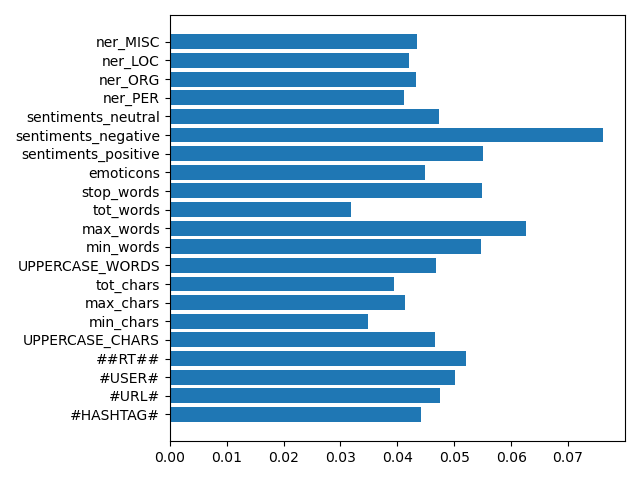
\includegraphics[width=0.75\textwidth]{assets/img/xgb_imp.png}
         \caption{\ac{XGB}}
         \label{fig:results:feat-imp::xgb}
         \vspace{0.6cm}
     \end{subfigure}
     \hfill
     \begin{subfigure}[b]{0.48\textwidth}
         \centering
         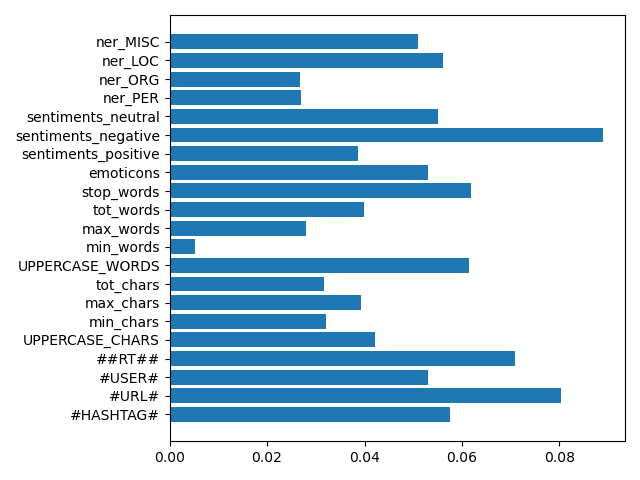
\includegraphics[width=\textwidth]{assets/img/rf_imp.png}
         \caption{\ac{RF}}
         \label{fig:results:feat-imp::rf}
     \end{subfigure}
     \hfill
     \begin{subfigure}[b]{0.48\textwidth}
         \centering
         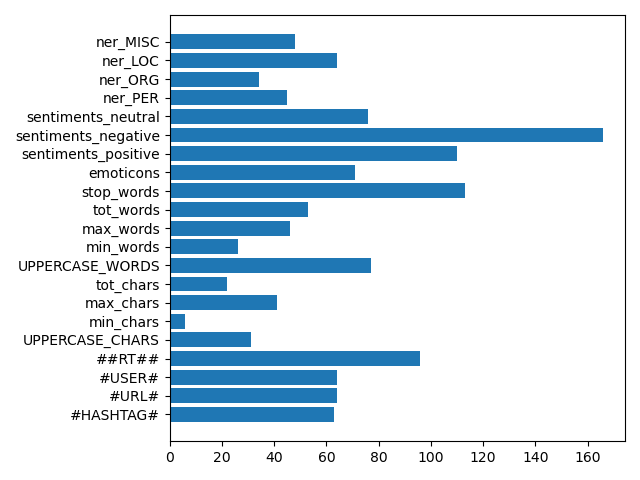
\includegraphics[width=\textwidth]{assets/img/lgb_imp.png}
         \caption{\ac{LGBM}}
         \label{fig:results:feat-imp::lgbm}
     \end{subfigure}
        \caption[Feature importance from trained \texorpdfstring{XGB}{XGB}, \texorpdfstring{RF}{RF} and \texorpdfstring{LGBM}{LGBM} models in Section \ref{sec:models:feat-based}]{Feature importance from trained \ac{XGB}, \ac{RF} and \ac{LGBM} models in Section \ref{sec:models:feat-based}}
        \label{fig:results:feat-imp}
\end{figure}
% https://tex.stackexchange.com/questions/551637/using-acronyms-in-toc

\newpage

\subsection{Word-embedding based representation}
\label{sec:results:word-emb}

% Please add the following required packages to your document preamble:
% \usepackage{multirow}
% \usepackage[table,xcdraw]{xcolor}
% If you use beamer only pass "xcolor=table" option, i.e. \documentclass[xcolor=table]{beamer}
\begin{table}[htbp]
\centering
\begin{tabular}{llrrrr}
\hline
\multicolumn{1}{l}{\textbf{Embedding}} &  & \multicolumn{1}{l}{} & \multicolumn{1}{l}{} & \multicolumn{1}{l}{} & \multicolumn{1}{l}{} \\
\multicolumn{1}{l}{\textbf{dimension}} & \multirow{-2}{*}{\textbf{Pooling}} & \multicolumn{1}{l}{\multirow{-2}{*}{\textbf{Accuracy}}} & \multicolumn{1}{l}{\multirow{-2}{*}{\textbf{Precision}}} & \multicolumn{1}{l}{\multirow{-2}{*}{\textbf{Recall}}} & \multicolumn{1}{l}{\multirow{-2}{*}{\textbf{F1-score}}} \\ \hline
 & Mean & 0.5200 & 0.5161 & 0.6400 & 0.5714 \\
 & Max. & 0.5200 & 0.5179 & 0.5800 & 0.5472 \\
 & Min. & 0.5500 & 0.5455 & 0.6000 & 0.5714 \\
\multirow{-4}{*}{25} & Abs. Max. & 0.5500 & 0.5556 & 0.5000 & 0.5263 \\ \hline
 & Mean & 0.4900 & 0.4923 & 0.6400 & 0.5565 \\
 & Max. & 0.4500 & 0.4444 & 0.4000 & 0.4211 \\
 & Min. & 0.5000 & 0.5000 & 0.5200 & 0.5098 \\
\multirow{-4}{*}{200} & Abs. Max. & 0.5100 & 0.5091 & 0.5600 & 0.5333 \\ \hline
\end{tabular}
\caption{Performance of models trained with Word-embedding based representation (Section \ref{sec:models:word-emb-based})}
\label{tab:results:performance-word-emb-based}
\end{table}


From Table \ref{tab:results:performance-word-emb-based}, we can observe that the models' performances are worse than the previous two setups. The fact that the training set is small (only 200 examples in training set) could be one of the reasons for not being able to train robust deep learning models from scratch.


\subsection{Counting number of hate tweets}
\label{sec:results:count-hate}

As the first step, we train the ML models using the training set of HatEval and Zeerak's datasets and test the performance on their corresponding test sets. Then, we combine the training set of Hatval and Zeerak's datasets, train the ML models on the combined training set, and test the performance of each test set separately. We tabulate the results in Table \ref{tab:results:performance-count-hate}. 


% Please add the following required packages to your document preamble:
% \usepackage{multirow}
\begin{table}[htbp]
\centering
\begin{tabular}{p{2cm}p{2cm}lrrrr}
\hline
\textbf{Training data} & \textbf{Test data} & \textbf{Model} & \multicolumn{1}{l}{\textbf{Accuracy}} & \multicolumn{1}{l}{\textbf{Precision}} & \multicolumn{1}{l}{\textbf{Recall}} & \multicolumn{1}{l}{\textbf{F1-score}} \\
\hline
\multirow{6}{*}{HatEval} & \multirow{6}{*}{HatEval} & LR & 0.4507 & 0.4280 & 0.9151 & 0.5832 \\
 &  & SVM & 0.4470 & 0.4259 & 0.9103 & 0.5803 \\
 &  & NB & \textbf{0.4763} & 0.4044 & 0.5222 & 0.4558 \\
 &  & RF & 0.4640 & 0.4343 & 0.9135 & 0.5887 \\
 &  & XGB & 0.4740 & 0.4388 & 0.9040 & 0.5908 \\
 &  & LGBM & 0.4637 & 0.4337 & 0.9056 & 0.5865 \\ \hline
\multirow{6}{*}{Zeerak's} & \multirow{6}{*}{Zeerak's} & LR & 0.6586 & 0.4744 & 0.6243 & 0.5391 \\
 &  & SVM & 0.6889 & 0.5110 & 0.6383 & 0.5676 \\
 &  & NB & 0.5630 & 0.3865 & 0.6235 & 0.4772 \\
 &  & RF & \textbf{0.7014} & 0.5237 & 0.7345 & 0.6115 \\
 &  & XGB & 0.7012 & 0.5239 & 0.7204 & 0.6067 \\
 &  & LGBM & 0.6993 & 0.5213 & 0.7322 & 0.6090 \\ \hline
\multirow{6}{*}{\parbox{2cm}{HatEval + Zeerak's}} & \multirow{6}{*}{HatEval} & LR & 0.4813 & 0.4296 & 0.7167 & 0.5372 \\
 &  & SVM & 0.4820 & 0.4323 & 0.7444 & 0.5469 \\
 &  & NB & 0.4740 & 0.4058 & 0.5437 & 0.4647 \\
 &  & RF & 0.4857 & 0.4332 & 0.7286 & 0.5434 \\
 &  & XGB & \textbf{0.5007} & 0.4430 & 0.7341 & 0.5526 \\
 &  & LGBM & 0.4850 & 0.4315 & 0.7119 & 0.5373 \\ \hline
\multirow{6}{*}{\parbox{2cm}{HatEval + Zeerak's}} & \multirow{6}{*}{Zeerak's} & LR & 0.5940 & 0.4170 & 0.6768 & 0.5161 \\
 &  & SVM & 0.5848 & 0.4165 & 0.7433 & 0.5339 \\
 &  & NB & 0.5571 & 0.3647 & 0.5185 & 0.4282 \\
 &  & RF & \textbf{0.6749} & 0.4946 & 0.7448 & 0.5945 \\
 &  & XGB & 0.6712 & 0.4910 & 0.7700 & 0.5997 \\
 &  & LGBM & 0.6695 & 0.4893 & 0.7604 & 0.5954 \\ \hline
\end{tabular}
\caption{Performance of models trained for classifying the tweets in Section \ref{sec:models:count-hate}}
\label{tab:results:performance-count-hate}
\end{table}

The models trained on the Zeerak's dataset seem to have significantly better performance than those trained on the HatEval dataset. For instance, the best performing model for the Zeerak's dataset, \ac{RF}, got an accuracy of 70.14\% on the test set. \ac{XGB} is also close with an accuracy of 70.12\%. On the other hand, the accuracy of the models trained on HatEval is less than 50\%. We investigate the poor performance of the models on the HatEval dataset. We evaluate them on the validation set of the HatEval dataset. Note that we performed the 10-fold cross-validation on the training set only and that the validation set was not used at any point. We tabulate the results in Table \ref{tab:results:performance-count-hate:val}.

% Please add the following required packages to your document preamble:
% \usepackage{multirow}
\begin{table}[htbp]
\centering
\begin{tabular}{p{2cm}llrrrr}
\hline
\textbf{Training data} & \textbf{Test data} & \textbf{Model} & \multicolumn{1}{l}{\textbf{Accuracy}} & \multicolumn{1}{l}{\textbf{Precision}} & \multicolumn{1}{l}{\textbf{Recall}} & \multicolumn{1}{l}{\textbf{F1-score}} \\ \hline
\multirow{6}{*}{HatEval} & \multirow{6}{*}{\begin{tabular}[c]{@{}l@{}}Validation set\\  of HatEval\end{tabular}} & LR & 0.6640 & 0.5697 & 0.8712 & 0.6889 \\
 &  & SVM & 0.6660 & 0.5784 & 0.8033 & 0.6725 \\
 &  & NB & 0.5820 & 0.5128 & 0.4215 & 0.4627 \\
 &  & RF & 0.6550 & 0.5693 & 0.7892 & 0.6614 \\
 &  & XGB & 0.6700 & 0.5826 & 0.8009 & 0.6746 \\
 &  & LGBM & 0.6540 & 0.5667 & 0.8056 & 0.6654 \\ \hline
\multirow{6}{*}{\parbox{2cm}{HatEval + Zeerak's}} & \multirow{6}{*}{\begin{tabular}[c]{@{}l@{}}Validation set\\  of HatEval\end{tabular}} & LR & 0.6270 & 0.5474 & 0.7307 & 0.6259 \\
 &  & SVM & 0.6220 & 0.5467 & 0.6721 & 0.6029 \\
 &  & NB & 0.6170 & 0.5570 & 0.5035 & 0.5289 \\
 &  & RF & 0.6220 & 0.5476 & 0.6604 & 0.5987 \\
 &  & XGB & 0.6500 & 0.5750 & 0.6909 & 0.6277 \\
 &  & LGBM & 0.6350 & 0.5620 & 0.6581 & 0.6063 \\ \hline
\end{tabular}
\caption{Performance of models on the validation set of the HatEval dataset, trained for classifying the tweets in Section \ref{sec:models:count-hate}}
\label{tab:results:performance-count-hate:val}
\end{table}

The accuracy looks far better than that obtained with the test set, with \ac{XGB} having an accuracy of up to 67\% when trained only with the HatEval dataset and 65\% when trained with the combined dataset. Additionally, we also observed a similar performance gap between the validation set and the test set in the paper submitted by the FERMI team \cite{fermi}, the top-performing team in the competition. Their best performing model had an accuracy of 65\% on the test set but only 57.13\% on the validation set, while the best accuracy achieved on the validation set was 71.18\%. Such a difference is most probably due to the difference between the distributions in the validation and the test sets.

Another interesting observation from Tables \ref{tab:results:performance-count-hate} and \ref{tab:results:performance-count-hate:val} is that the performance has also dropped when more data is added. For instance, the performance of the models trained only on the Zeerak's dataset is higher than those trained on the combined dataset. A similar trend can be seen in the case of the performance of models on the validation set of the HatEval dataset, i.e., the performance of the models trained only on the HatEval dataset is higher than those trained on the combined dataset. Hence, more data does not always mean better performance-- the quality of the data is also important. In this case, this probably occurs because the data in both these datasets come from different distributions. 


% % Please add the following required packages to your document preamble:
% % \usepackage{multirow}
% \begin{table}[htbp]
% \centering
% \begin{tabular}{p{2cm}p{2cm}lrrrr}
% \hline
% \textbf{Training data} & \textbf{Test data} & \textbf{Model} & \multicolumn{1}{l}{\textbf{Accuracy}} & \multicolumn{1}{l}{\textbf{Precision}} & \multicolumn{1}{l}{\textbf{Recall}} & \multicolumn{1}{l}{\textbf{F1-score}} \\ \hline
% \multirow{6}{*}{\parbox{2cm}{HatEval (Train+Val)}} & \multirow{6}{*}{\parbox{2cm}{HatEval (Test)}} & LR & 0.4520 & 0.4287 & 0.9167 & 0.5842 \\
%  &  & SVM & 0.4477 & 0.4264 & 0.9127 & 0.5812 \\
%  &  & NB & 0.4740 & 0.4038 & 0.5294 & 0.4581 \\
%  &  & RF & 0.4523 & 0.4288 & 0.9151 & 0.5839 \\
%  &  & XGB & 0.4593 & 0.4318 & 0.9095 & 0.5856 \\
%  &  & LGBM & 0.4583 & 0.4312 & 0.9079 & 0.5847 \\ \hline
% \end{tabular}
% \caption{Performance of models on test set of HatEval trained on training and validation set of HatEval (Section \ref{sec:models:count-hate})}
% \label{tab:results:performance-count-hate:train+val}
% \end{table}

We now move to the next stage of getting the prediction for a user based on the number of tweets containing Hate Speech. We choose one model from each of the three training data setups in Table \ref{tab:results:performance-count-hate}. In particular, we choose \ac{RF} for the Zeerak's dataset case (the best performing model) and \ac{XGB} for the HatEval case (the best model after \ac{NB}) and the combined dataset case (the best model on the HatEval's test set and second, yet close to the first, on the Zeerak's test set). We also include the fine-tuned transformer-based \ac{RoBERTa} model described in Section \ref{sec:models:count-hate}.

We move back to the PAN @ CLEF 2021 dataset and get the hate scores for each tweet. We now need to determine the ``threshold'', which will determine the minimum number of Hate Speech containing tweets to be present to flag the user as a Hate Speech Spreader. This value is determined by iterating over different values (ideally from 1 to 200, in our case) and choosing the one that gives the best results on the training set. We perform this experiment with the models mentioned above and report the results, along with the best threshold value determined, in Table \ref{tab:results:performance-count-hate:main}.





% Please add the following required packages to your document preamble:
% \usepackage[table,xcdraw]{xcolor}
% If you use beamer only pass "xcolor=table" option, i.e. \documentclass[xcolor=table]{beamer}
% \usepackage[normalem]{ulem}
% \useunder{\uline}{\ul}{}
\begin{table}[htbp]
\centering
\begin{tabular}{p{1.9cm}\eat{ p{2.05cm}}p{2.2cm}rrrrr}
\hline
\textbf{Training data} \eat{& \textbf{Test data}} & \textbf{Model} & \multicolumn{1}{l}{\textbf{Accuracy}} & \multicolumn{1}{l}{\textbf{Precision}} & \multicolumn{1}{l}{\textbf{Recall}} & \multicolumn{1}{l}{\textbf{F1-score}} & \multicolumn{1}{l}{Threshold} \\ \hline
HatEval \eat{& PAN @ CLEF 2021} & XGB & 0.5400 & 0.5357 & 0.6000 & 0.5660 & 80 \\
Zeerak's \eat{& PAN @ CLEF 2021} & RF & 0.4800 & 0.4808 & 0.5000 & 0.4902 & 60 \\
HatEval + Zeerak's \eat{& PAN @ CLEF 2021} & XGB & 0.5800 & 0.5714 & 0.6400 & 0.6038 & 80 \\ \hline
{---} \eat{& PAN @ CLEF 2021} & {\texttt{cardiffnlp/ twitter- roberta-base- hate}} & \textbf{0.6900} & 0.8065 & 0.5000 &  {0.6173} & 10 \\ \hline
\end{tabular}
\caption{Performance obtained by counting the number of Hate Speech containing tweets (Section \ref{sec:models:count-hate})}
\label{tab:results:performance-count-hate:main}
\end{table}

It can be observed that the system using the \ac{RoBERTa} model for obtaining the tweet scores has the best accuracy of 69\% on the test set. We also obtained the same accuracy with Term-frequency based representation baselines in Section \ref{sec:results:tf-idf}. It flags any user as Hate Speech Spreader if they have posted at least ten tweets containing Hate Speech. It is also interesting to note that this number is similar to the threshold used for annotating the users during dataset preparation (Section \ref{sec:dataset:overview}).

\section{Our Model}
\label{sec:results:our-model}

\ac{GloVe} Twitter consists of word embeddings in four different dimensions-- 25d, 50d, 100d and 200d. Usually, the smaller dimensional ones are useful for syntactic tasks, and the larger ones are useful for semantic tasks. However, which one is most suitable can be determined only through experiments and hence, we present the performance of our proposed models for all the four dimensions in Table \ref{tab:results:performance-our-model} and plot their accuracies in Figure \ref{fig:results:performance-our-model}.

% Please add the following required packages to your document preamble:
% \usepackage{multirow}
\begin{table}[htbp]
\centering
\begin{tabular}{llrrrr}
\hline
\textbf{Embedding} & \textbf{Model} & \multicolumn{1}{l}{\textbf{Accuracy}} & \multicolumn{1}{l}{\textbf{Precision}} & \multicolumn{1}{l}{\textbf{Recall}} & \multicolumn{1}{l}{\textbf{F1-score}} \\
\textbf{dimension (d)} &  & \multicolumn{1}{l}{} & \multicolumn{1}{l}{} & \multicolumn{1}{l}{} & \multicolumn{1}{l}{} \\ \hline
\multirow{6}{*}{25} & LR & \textbf{0.7600} & 0.7407 & 0.8000 & 0.7692 \\
 & SVM & 0.7300 & 0.7255 & 0.7400 & 0.7327 \\
 & RF & 0.6800 & 0.6667 & 0.7200 & 0.6923 \\
 & XGB & 0.6500 & 0.6415 & 0.6800 & 0.6602 \\
 & LGBM & 0.6900 & 0.6792 & 0.7200 & 0.6990 \\
 & NN & 0.6000 & 0.5962 & 0.6200 & 0.6078 \\ \cline{2-6} 
\multirow{6}{*}{50} & LR & 0.7200 & 0.7037 & 0.7600 & 0.7308 \\
 & SVM & 0.7200 & 0.7115 & 0.7400 & 0.7255 \\
 & RF & \textbf{0.7300} & 0.7170 & 0.7600 & 0.7379 \\
 & XGB & 0.7200 & 0.6897 & 0.8000 & 0.7407 \\
 & LGBM & 0.7200 & 0.6964 & 0.7800 & 0.7358 \\
 & NN & 0.6400 & 0.6250 & 0.7000 & 0.6604 \\ \hline
\multirow{6}{*}{100} & LR & 0.7100 & 0.6981 & 0.7400 & 0.7184 \\
 & SVM & 0.6900 & 0.6792 & 0.7200 & 0.6990 \\
 & RF & 0.7100 & 0.7234 & 0.6800 & 0.7010 \\
 & XGB & \textbf{0.7200} & 0.7391 & 0.6800 & 0.7083 \\
 & LGBM & 0.7000 & 0.7273 & 0.6400 & 0.6809 \\
 & NN & 0.7100 & 0.6721 & 0.8200 & 0.7387 \\ \hline
\multirow{6}{*}{200} & LR & 0.7100 & 0.6842 & 0.7800 & 0.7290 \\
 & SVM & 0.7200 & 0.6897 & 0.8000 & 0.7407 \\
 & RF & \textbf{0.7500} & 0.7193 & 0.8200 & 0.7664 \\
 & XGB & 0.7200 & 0.7037 & 0.7600 & 0.7308 \\
 & LGBM & 0.7100 & 0.6981 & 0.7400 & 0.7184 \\
 & NN & 0.6900 & 0.6610 & 0.7800 & 0.7156 \\ \cline{2-6} 
\end{tabular}
\caption[Performance of our proposed models (Section \ref{sec:models:our-model}) for different \texorpdfstring{GloVe}{GloVe} word embedding dimensions]{Performance of our proposed models (Section \ref{sec:models:our-model}) for different \ac{GloVe} word embedding dimensions}
\label{tab:results:performance-our-model}
\end{table}

\begin{figure}[htbp]
    \centering
    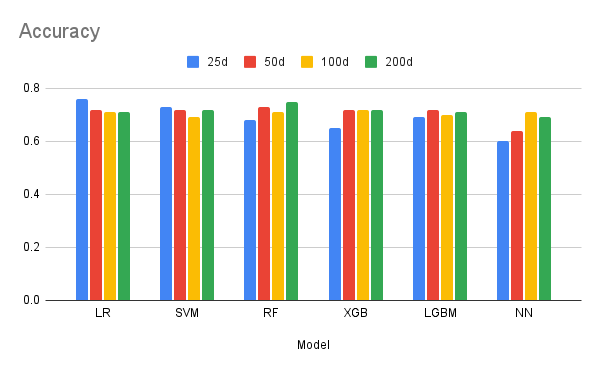
\includegraphics[width=0.9\textwidth]{assets/img/our-model_all.png}
    \caption[Accuracies of our proposed models (Section \ref{sec:models:our-model}) for different \texorpdfstring{GloVe}{GloVe} word embedding dimensions]{Accuracies of our proposed models (Section \ref{sec:models:our-model}) for different \ac{GloVe} word embedding dimensions}
    \label{fig:results:performance-our-model}
\end{figure}

It can be observed that many of these models have outperformed our previous baselines. \ac{LR} with 25d \ac{GloVe} word embeddings has obtained the best performance with an accuracy of 76\% and an F1-score of 76.92\% on the test set. Among the 50d, 100d and 200d word embeddings setup, the best performing models in terms of accuracy are \ac{RF}, \ac{XGB} and \ac{RF} respectively. The best performing model has 7\% more accuracy than our best baseline models. It has also outperformed the best model in the competition by 1\%.

\paragraph{Comparing the models without using a weighted sum:} 
We are interested in studying if introducing the sentiment scores as weights have actually helped improve the performance. To test this out, we build very similar models, except that we take the weight to be ``\textit{one}'' for all the words, i.e., we take an unweighted sum in Step \ref{enum:models:our-model:method:wght-sum} of the process (Section \ref{sec:models:our-model:methodology}). We present the results in the case of 25d \ac{GloVe} word embeddings only (the setup in which the best performance was obtained) in Table \ref{tab:results:performance-our-model:unweighted}. We also plot the accuracies for easier comparision in Figure \ref{fig:results:performance-our-model:unweighted}. It can be observed that the performance drops significantly when the weighted sum is replaced with an unweighted sum. This shows that the introduction of sentiment scores as weights is useful. 

% Please add the following required packages to your document preamble:
% \usepackage{multirow}
\begin{table}[htbp]
\centering
\begin{tabular}{llrrrr}
\hline
\multicolumn{1}{l}{\textbf{Setup}} & \textbf{Model} & \multicolumn{1}{l}{\textbf{Accuracy}} & \multicolumn{1}{l}{\textbf{Precision}} & \multicolumn{1}{l}{\textbf{Recall}} & \multicolumn{1}{l}{\textbf{F1-score}} \\ \hline
\multirow{6}{*}{\begin{tabular}[c]{@{}l@{}}Our Model \\ (weighted sum)\end{tabular}} & LR & 0.7600 & 0.7407 & 0.8000 & 0.7692 \\
 & SVM & 0.7300 & 0.7255 & 0.7400 & 0.7327 \\
 & RF & 0.6800 & 0.6667 & 0.7200 & 0.6923 \\
 & XGB & 0.6500 & 0.6415 & 0.6800 & 0.6602 \\
 & LGBM & 0.6900 & 0.6792 & 0.7200 & 0.6990 \\
 & NN & 0.6000 & 0.5962 & 0.6200 & 0.6078 \\ \hline
\multirow{6}{*}{Unweighted sum} & LR & 0.6400 & 0.6296 & 0.6800 & 0.6538 \\
 & SVM & 0.6500 & 0.6316 & 0.7200 & 0.6729 \\
 & RF & 0.6500 & 0.6531 & 0.6400 & 0.6465 \\
 & XGB & 0.6000 & 0.6000 & 0.6000 & 0.6000 \\
 & LGBM & 0.6600 & 0.6538 & 0.6800 & 0.6667 \\
 & NN & 0.6300 & 0.6667 & 0.5200 & 0.5843 \\ \cline{2-6} 
\end{tabular}
\caption{Comparing the performance of our proposed models (Section \ref{sec:models:our-model}) when the weighted sum of sentiment scores is replaced with an unweighted sum}
\label{tab:results:performance-our-model:unweighted}
\end{table}

\begin{figure}[htbp]
    \centering
    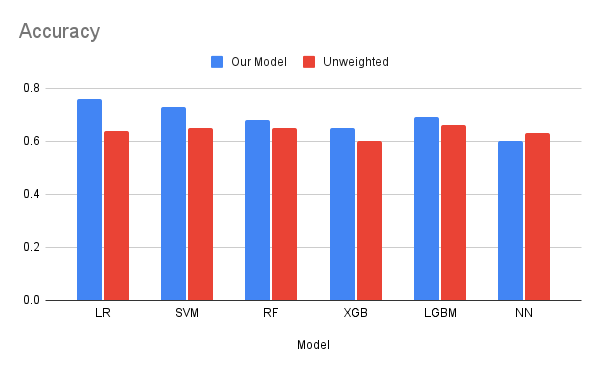
\includegraphics[width=0.8\textwidth]{assets/img/our-model_unweight.png}
    \caption{Comparing the accuracies of our proposed models (Section \ref{sec:models:our-model}) when the weighted sum of sentiment scores is replaced with an unweighted sum}
    \label{fig:results:performance-our-model:unweighted}
\end{figure}

\paragraph{Ablation study:}
We make minor modifications in the model setup and observe how the performance changes with these modifications. In particular, we do the following: (i) do not perform stopwords removal in Step \ref{enum:models:our-model:method:stopwords} (denoted as ``\textit{-stopwords removal}''); (ii) use the lemmatized or stemmed form of the word if it is not found in one of the SentiWordNet or \ac{GloVe} vocabulary, if the lemmatized/stemmed forms are present, in Step \ref{enum:models:our-model:method:swn-embd} (denoted as ``\textit{+lemmatization +stemming}''); and (iii) use max-pooling, i.e., taking maximum value in each dimension, to aggregate the tweet representations and obtain a user representation in Step \ref{enum:models:our-model:method:wght-sum} (denoted as ``\textit{max-pooling}''). Note that we only perform one of these modifcations at a time. We tabulate the performance in the case of 25d \ac{GloVe} word embeddings only (the setup in which the best performance was obtained) in Table \ref{tab:results:performance-our-model:abl}. We plot the accuracies in Figure \ref{fig:results:performance-our-model:abl}.
At least one of the positive, neutral or negative sentiment scores is non-zero for a word (in fact, they sum up to one). Hence, not removing the stopwords adds noise to some dimensions of the user representation, which might be the probable reason for the drop in performance.{Moreover, some sentiments carrying words like ``very'' are included in the list of stopwords.}
Using the lemmatized or stemmed forms of the words must help incorporate some of the OOV words. However, we can also observe performance drops in some of the classifiers. Further investigation might be required before concluding in this regard.
We can also observe a significant drop in performance when mean-pooling is replaced with max-pooling for aggregating the tweet representations.


% Please add the following required packages to your document preamble:
% \usepackage{multirow}
\begin{table}[htbp]
\centering
\begin{tabular}{p{3cm}lrrrr}
\hline
\textbf{Ablation} & \textbf{Model} & \multicolumn{1}{l}{\textbf{Accuracy}} & \multicolumn{1}{l}{\textbf{Precision}} & \multicolumn{1}{l}{\textbf{Recall}} & \multicolumn{1}{l}{\textbf{F1-score}} \\ \hline
\multirow{6}{*}{N/A} & LR & 0.7600 & 0.7407 & 0.8000 & 0.7692 \\
 & SVM & 0.7300 & 0.7255 & 0.7400 & 0.7327 \\
 & RF & 0.6800 & 0.6667 & 0.7200 & 0.6923 \\
 & XGB & 0.6500 & 0.6415 & 0.6800 & 0.6602 \\
 & LGBM & 0.6900 & 0.6792 & 0.7200 & 0.6990 \\
 & NN & 0.6000 & 0.5962 & 0.6200 & 0.6078 \\ \hline
\multirow{6}{*}{\parbox{3cm}{-stopwords  \ \ \ \ \ \ \ \ removal}} & LR & 0.7300 & 0.7170 & 0.7600 & 0.7379 \\
 & SVM & 0.6800 & 0.6552 & 0.7600 & 0.7037 \\
 & RF & 0.6500 & 0.6596 & 0.6200 & 0.6392 \\
 & XGB & 0.6700 & 0.6809 & 0.6400 & 0.6598 \\
 & LGBM & 0.6500 & 0.6415 & 0.6800 & 0.6602 \\
 & NN & 0.6400 & 0.6296 & 0.6800 & 0.6538 \\ \hline
\multirow{6}{*}{\parbox{3cm}{+lemmatization +stemming}} & LR & 0.7200 & 0.6964 & 0.7800 & 0.7358 \\
 & SVM & 0.7200 & 0.7115 & 0.7400 & 0.7255 \\
 & RF & 0.7100 & 0.6981 & 0.7400 & 0.7184 \\
 & XGB & 0.7000 & 0.6786 & 0.7600 & 0.7170 \\
 & LGBM & 0.6700 & 0.6349 & 0.8000 & 0.7080 \\
 & NN & 0.6800 & 0.6607 & 0.7400 & 0.6981 \\ \hline
\multirow{6}{*}{\parbox{3cm}{max-pooling}} & LR & 0.5700 & 0.5745 & 0.5400 & 0.5567 \\
 & SVM & 0.5800 & 0.5833 & 0.5600 & 0.5714 \\
 & RF & 0.6400 & 0.6296 & 0.6800 & 0.6538 \\
 & XGB & 0.6100 & 0.6170 & 0.5800 & 0.5979 \\
 & LGBM & 0.5800 & 0.5690 & 0.6600 & 0.6111 \\
 & NN & 0.5600 & 0.5500 & 0.6600 & 0.6000 \\ \hline
\end{tabular}
\caption{Performance of our proposed models (Section \ref{sec:models:our-model}) with ablations: (i) stopwords removal; (ii) using lemmatized/stemmed form of an OOV word; and (iii) max-pooling}
\label{tab:results:performance-our-model:abl}
\end{table}

\begin{figure}[htbp]
    \centering
    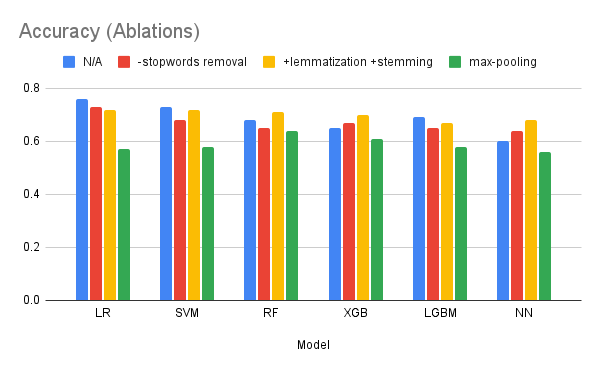
\includegraphics[width=0.9\textwidth]{assets/img/our-model_ablations.png}
    \caption{Accuracies of our proposed models (Section \ref{sec:models:our-model}) with ablations: (i) stopwords removal; (ii) using lemmatized/stemmed form of an OOV word; and (iii) max-pooling}
    \label{fig:results:performance-our-model:abl}
\end{figure}

\section{Ensemble}
\label{sec:results:ensemble}
Clearly, the fine-tuned \ac{RoBERTa} model and the \ac{LR} classifier with 25d \ac{GloVe} word embeddings have the best performance in Section \ref{sec:results:count-hate} and Section \ref{sec:results:our-model}, respectively. However, since both \ac{TF-IDF}+\ac{LR} and \ac{TF-IDF}+\ac{SVM} have the same test accuracy in Section \ref{sec:results:tf-idf}, we create two different ensembles, including one in each. Hence, we have two max-voting classifiers: (i) \ac{TF-IDF}/\ac{LR} + \ac{RoBERTa} + 25d/\ac{LR}; and (ii) \ac{TF-IDF}/\ac{SVM} + \ac{RoBERTa} + 25d/\ac{LR}. Their performance on the test set is tabulated in Table \ref{tab:results:performance-ensemble}. 

\begin{table}[htbp]
\centering
\begin{tabular}{lrrrr}
\hline
\textbf{Model} & \multicolumn{1}{l}{\textbf{Accuracy}} & \multicolumn{1}{l}{\textbf{Precision}} & \multicolumn{1}{l}{\textbf{Recall}} & \multicolumn{1}{l}{\textbf{F1-score}} \\ \hline
TF-IDF/LR + RoBERTa + 25d/LR & \textbf{0.7700} & 0.8000 & 0.7200 & {0.7579} \\
TF-IDF/SVM + RoBERTa + 25d/LR & 0.7600 & 0.7708 & 0.7400 & 0.7551 \\ \hline
\end{tabular}
\caption{Performance of ensemble models (Section \ref{sec:models:ensemble})}
\label{tab:results:performance-ensemble}
\end{table}

We can observe that \ac{TF-IDF}/\ac{LR} + \ac{RoBERTa} + 25d/\ac{LR} has achieved an accuracy of 77\% on the test set, which is a further 1\% increase from the standalone 25d/\ac{LR} model.

\section{Error Analysis}
\label{sec:results:err-ana}

We perform a detailed error analysis only for the models we proposed (Section \ref{sec:models:our-model}) in this section.

% \subsection{Our Model}
% \label{sec:results:err-ana:our-model}

\paragraph{Sample OOV words:}
We drop those words that are not part of the SentiWordNet or \ac{GloVe} word embeddings vocabulary (in Step \ref{enum:models:our-model:method:swn-embd}). We collected a list of such most commonly occurring OOV words and manually classified them into two categories-- (i) containing internet slang or typos; and (ii) possibly hate carrying words. We tabulate them in Table \ref{tab:err-ana:our_model:oov}.
Some words are OOV because of invalid/incorrect POS tags obtained while parsing the tweets. Parsing tweets remains an active research area in NLP in itself, and hence, we do not move towards it further. We can also observe that most of the words in the second category are named-entity mentions (e.g., person names, locations, organizations, etc.). Even if we manually assign sentiment scores using heuristics, obtaining word embeddings will remain a challenge because it will require scratch training.


% \begin{table}[htbp]
% \centering
% \begin{tabular}{|p{6.4cm}|p{6.4cm}|}
% \hline
% Containing internet slang or typos & Possibly hate carrying words \\ \hline
% im, dont, thats, yall, lol, aint, youre, cant, gt, gotta, wanna, didnt, doesnt, hes, lets, ive, lmao, isnt, gonna, rt, retweet, theyre, yo, whats, bro, ya, shes, ima, theres, lil, ppl, wasnt, tryna, wont, ur, arent, wouldnt, dems, oh, uk, dr, havent, heres, cuz, couldnt, idk, nah, finna, omg, whos, gon, youll, blm, smh, usa, youtube, tweets, w, vs, bruh, idc, imma, eu, twitter, ca, id, youve, bc, shouldnt, outta, lmfao, thru, yep, til, hasnt, lmaoo, lt, gov, fbi, dem, shouldve, gf, goin, gf, goin & biden, women, niggas, thank, fucking, followed, nigga, joe, covid, democrats, fuck, media, unfollowed, bitches, shit, friends, americans, america, donald, children, guys, states, tf, wtf, obama, fucked, pelosi, girls, bbc, facebook, cuomo, trumps, god, tommy, republicans, trump, killed, voted, voters, coronavirus, sorry, af, mad, arrested, hoes, disgusting, follow, illegals, following, mfs, jews, antifa, muslims, asf, killing, whites, cnn, fuckin, liberals, boys, patriots, girl, migrants, cute, trans, elections, cops, immigrants, hillary, guns, chris, meghan, blacks, protesters, womens, dennis, females, politicians, ass, babies, conservatives, dick, boy, maga, racist  \\ \hline
% \end{tabular}
% \caption{Sample OOV words for our model}
% \label{tab:err-ana:our_model:oov}
% \end{table}

% \begin{table}[htbp]
% \centering
% \begin{tabular}{|p{6.8cm}|p{8.5cm}|}
% \hline
% \textbf{Containing internet slang/typos} & \textbf{Possibly hate carrying words} \\ \hline
% im, dont, thats, yall, lol, aint, youre, cant, gt, gotta, wanna, didnt, doesnt, hes, lets, ive, lmao, isnt, gonna, rt, theyre, yo, whats, bro, ya, shes, ima, theres, lil, ppl, wasnt, tryna, wont, ur, arent, wouldnt, dems, oh, uk, dr, havent, heres, cuz, couldnt, idk, nah, finna, omg, whos, gon, youll, blm, smh, w, vs, bruh, idc, imma, id, youve, shouldnt, outta, lmfao, thru, yep, til, hasnt, lmaoo, lt, gov, fbi, dem, shouldve, gf, goin, gf, goin & biden, women, niggas, fucking, nigga, joe, covid, democrats, fuck, media, bitches, shit, friends, americans, america, donald, children, guys, states, tf, wtf, obama, fucked, pelosi, girls, bbc, facebook, cuomo, trumps, god, tommy, republicans, trump, killed, voted, voters, coronavirus, sorry, af, mad, arrested, hoes, disgusting, illegals, following, mfs, jews, antifa, muslims, asf, whites, cnn, fuckin, liberals, boys, patriots, girl, migrants, elections, cops, immigrants, hillary, guns, chris, meghan, blacks, protesters, womens, females, politicians, ass, babies, conservatives, dick, boy, maga, racist  \\ \hline
% \end{tabular}
% \caption{Sample OOV words for our model}
% \label{tab:err-ana:our_model:oov}
% \end{table}




% \begin{table}[htbp]
% \centering
% \begin{tabular}{|p{6.8cm}|p{8.5cm}|}
% \hline
% \textbf{Containing internet slang/typos} & \textbf{Possibly hate carrying words} \\ \hline
% im, dont, thats, yall, lol, aint, youre, cant, gt, gotta, wanna, didnt, doesnt, hes, lets, ive, lm\*o, isnt, gonna, rt, theyre, yo, whats, bro, ya, shes, ima, theres, lil, ppl, wasnt, tryna, wont, ur, arent, wouldnt, dems, oh, uk, dr, havent, heres, cuz, couldnt, idk, nah, finna, omg, whos, gon, youll, blm, smh, w, vs, bruh, idc, imma, id, youve, shouldnt, outta, lm\*\*o, thru, yep, til, hasnt, lm\*oo, lt, gov, fbi, dem, shouldve, gf, goin, gf, goin & biden, women, n\@\#\$as, f\@\#king, n\@\#\$a, joe, covid, democrats, f\@\#k, media, b\@\#\$hes, sh\*t, friends, americans, america, donald, children, guys, states, t\*, wt\*, obama, f\@\#ked, pelosi, girls, bbc, facebook, cuomo, trumps, god, tommy, republicans, trump, killed, voted, voters, coronavirus, sorry, a\*, mad, arrested, h\@\#s, disgusting, illegals, following, m\*s, jews, antifa, muslims, as\*, whites, cnn, f\@\#kin, liberals, boys, patriots, girl, migrants, elections, cops, immigrants, hillary, guns, chris, meghan, blacks, protesters, womens, females, politicians, a\*s, babies, conservatives, d\@\#k, boy, racist  \\ \hline
% \end{tabular}
% \caption{Sample OOV words for our model}
% \label{tab:err-ana:our_model:oov}
% \end{table}

\begin{table}[htbp]
\centering
\begin{tabular}{|p{6.8cm}|p{8.5cm}|}
\hline
\textbf{Containing internet slang/typos} & \textbf{Possibly hate carrying words} \\ \hline
im, dont, thats, yall, lol, aint, youre, cant, gt, gotta, wanna, didnt, doesnt, hes, lets, ive, lm*o, isnt, gonna, rt, theyre, yo, whats, bro, ya, shes, ima, theres, lil, ppl, wasnt, tryna, wont, ur, arent, wouldnt, dems, oh, uk, dr, havent, heres, cuz, couldnt, idk, nah, finna, omg, whos, gon, youll, blm, smh, w, vs, bruh, idc, imma, id, youve, shouldnt, outta, lm**o, thru, yep, til, hasnt, lm*oo, lt, gov, fbi, dem, shouldve, gf, goin, gf, goin & biden, women, n, as, f**king, n***a, joe, covid, democrats, f**k, media, b***hes, sh*t, friends, americans, america, donald, children, guys, states, t*, wt*, obama, f**ked, pelosi, girls, bbc, facebook, cuomo, trumps, god, tommy, republicans, trump, killed, voted, voters, coronavirus, sorry, a*, mad, arrested, h**s, disgusting, illegals, following, m*s, jews, antifa, muslims, as*, whites, cnn, f**kin, liberals, boys, patriots, girl, migrants, elections, cops, immigrants, hillary, guns, chris, meghan, blacks, protesters, womens, females, politicians, a*s, babies, conservatives, d**k, boy, racist  \\ \hline
\end{tabular}
\caption{Sample OOV words for our model}
\label{tab:err-ana:our_model:oov}
\end{table}

\paragraph{Confusion matrix:}
We plot the confusion matrix for the \ac{LR} model with 25d \ac{GloVe} word embeddings, which had the best performance in Section \ref{sec:results:our-model}, in Figure \ref{fig:err-ana:our_model:confusion}. We observe that 14 users have been classified as Hate Speech Spreaders even though they are not (False Positives). 10 users have been classified as non-Hate Speech Spreaders even though they are (False Negatives).

\begin{figure}[htbp]
    \centering
    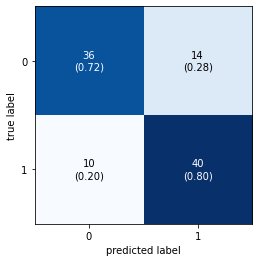
\includegraphics{assets/img/confusion_our-model.png}
    \caption{Confusion matrix of our best performing model\eat{ (Section \ref{sec:models:our-model})}}
    \label{fig:err-ana:our_model:confusion}
\end{figure}


\paragraph{Number of tweets with abusive word mentions:}
Among the misclassified users, we find the number of tweets that contain the usage of abusive words. We use the list of abusive words from a GitHub repository\footnote{\url{https://github.com/manoelhortaribeiro/HatefulUsersTwitter/blob/master/data/extra/bad_words.txt}} and tabulate the number of tweets that contain at least one, two and three abusive words for all the 24 users in Table \ref{tab:err-ana:our_model:abusive}.
Since the proportion of tweets containing abusive words is rather high for the 14 False Positive users, the proposed system wrongly labels them as positive. In a similar vein, the proportion of tweets having abusive words is relatively small for the 10 False Negative users and are therefore wrongly labelled as negative by our model.


% \hline
% \multicolumn{1}{c}{\textbf{\textgreater{}=1}} & \multicolumn{1}{c}{\textbf{\textgreater{}=2}} & \multicolumn{1}{c}{\textbf{\textgreater{}=3}} \\ \hline


% \begin{table}[htbp]
% \centering
% \begin{tabular}{rrr}
% \hline
% \multicolumn{1}{c}{\textbf{at least}} & \multicolumn{1}{c}{\textbf{at least}} & \multicolumn{1}{c}{\textbf{at least}} \\
% \multicolumn{1}{r}{\textbf{1}} & \multicolumn{1}{r}{\textbf{2}} & \multicolumn{1}{r}{\textbf{3}} \\ \hline
% \multicolumn{3}{r}{\textbf{False Positives}} \\ \hline
% 50 & 10 & 1 \\
% 41 & 5 & 0 \\
% 26 & 6 & 0 \\
% 51 & 9 & 3 \\
% 35 & 4 & 0 \\
% 16 & 0 & 0 \\
% 4 & 0 & 0 \\
% 12 & 1 & 0 \\
% 10 & 1 & 0 \\
% 11 & 1 & 0 \\
% 4 & 0 & 0 \\
% 29 & 5 & 0 \\
% 4 & 0 & 0 \\
% 17 & 3 & 0 \\ \hline
% \multicolumn{3}{c}{\textbf{False Negatives}} \\ \hline
% 2 & 0 & 0 \\
% 35 & 2 & 0 \\
% 1 & 0 & 0 \\
% 0 & 0 & 0 \\
% 4 & 0 & 0 \\
% 5 & 0 & 0 \\
% 23 & 4 & 0 \\
% 2 & 0 & 0 \\
% 1 & 0 & 0 \\
% 4 & 0 & 0 \\ \hline
% \end{tabular}
% \caption{Number of tweets with at least one, two and three abusive words for the misclassified users}
% \label{tab:err-ana:our_model:abusive}
% \end{table}


\begin{table}[htbp]
\centering
\begin{subtable}{0.4\textwidth}
\centering
\begin{tabular}{rrr}
\hline
\multicolumn{1}{c}{\textbf{at least}} & \multicolumn{1}{c}{\textbf{at least}} & \multicolumn{1}{c}{\textbf{at least}} \\
\multicolumn{1}{r}{\textbf{1}} & \multicolumn{1}{r}{\textbf{2}} & \multicolumn{1}{r}{\textbf{3}} \\ \hline
50 & 10 & 1 \\
41 & 5 & 0 \\
26 & 6 & 0 \\
51 & 9 & 3 \\
35 & 4 & 0 \\
16 & 0 & 0 \\
4 & 0 & 0 \\
12 & 1 & 0 \\
10 & 1 & 0 \\
11 & 1 & 0 \\
4 & 0 & 0 \\
29 & 5 & 0 \\
4 & 0 & 0 \\
17 & 3 & 0 \\ \hline
\end{tabular}
\caption{False Positives}
\end{subtable}
\begin{subtable}{0.4\textwidth}
\centering
\begin{tabular}{rrr}
\hline
\multicolumn{1}{c}{\textbf{at least}} & \multicolumn{1}{c}{\textbf{at least}} & \multicolumn{1}{c}{\textbf{at least}} \\
\multicolumn{1}{r}{\textbf{1}} & \multicolumn{1}{r}{\textbf{2}} & \multicolumn{1}{r}{\textbf{3}} \\ \hline
2 & 0 & 0 \\
35 & 2 & 0 \\
1 & 0 & 0 \\
0 & 0 & 0 \\
4 & 0 & 0 \\
5 & 0 & 0 \\
23 & 4 & 0 \\
2 & 0 & 0 \\
1 & 0 & 0 \\
4 & 0 & 0 \\ \hline
\end{tabular}
\caption{False Negatives}
\end{subtable}
\caption{Number of tweets with at least one, two and three abusive words for the misclassified users}
\label{tab:err-ana:our_model:abusive}
\end{table}

\paragraph{Samples of tweets from misclassified users:}
Among the misclassified users, we show a few tweets shared by two users; one was falsely classified as positive, and the other was falsely classified as negative in Table \ref{tab:err-ana:our_model:examples}.
In the case of the False Positive user, even though the user uses abusive words, it is not targeted toward a particular individual or group. The user uses it casually, and such instances do not count under Hate Speech. This is one of the weaknesses of our model, i.e., it is not entirely aware of the intent.
In the case of the False Negative user, a larger proportion of the tweets give updates for a show. However, specific tweets contain Hate Speech (e.g., the third one), but these are quite small in number. Hence, the model has misclassified the user. This is a limitation of any ML model.


% \begin{table}[htbp]
% \centering
% \begin{tabular}{p{7cm}p{1cm}p{7cm}}
% \hline
% \textbf{False Positive User} &  & \textbf{False Negative User} \\ \hline
% \#USER\# \#USER\# \#USER\# Bitch you know wtf I mean, actin like you can’t tell smh &  & JJ McCartyney Show 03-10-2021 3-5PM ET Wednesday \#URL\# via \#USER\# \\ \hline
% \#USER\# \#USER\# \#USER\# You didn’t tag me first but I’m in bitch ���� &  & JJ McCartney previews today's special 7th Anniversary special!! \#URL\# via \#USER\# \\ \hline
% My mood is shit when my mind is in the wrong place &  & \#USER\# Cory Booker is a lying sack of crap. Terrori/hate crimes committed by whites/bigots? Prove it, you scumbag. \\ \hline
% Fucking hate doing shit last min ���� &  & IQ Al Rassooli is JJ's guest LIVE from 3 to 5pm ET on The JJ McCartney Show \#HASHTAG\# \#HASHTAG\# \#USER\# \#URL\# \\ \hline
% \end{tabular}
% \caption{Some samples of tweets made by two misclassified users}
% \label{tab:err-ana:our_model:examples}
% \end{table}



% \begin{table}[htbp]
% \centering
% \begin{tabular}{p{7cm}p{1cm}p{7cm}}
% \hline
% \textbf{False Positive User} &  & \textbf{False Negative User} \\ \hline
% \#USER\# \#USER\# \#USER\# B\@\#\$h you know wt\* I mean, actin like you can’t tell smh &  & JJ McCartyney Show 03-10-2021 3-5PM ET Wednesday \#URL\# via \#USER\# \\ \hline
% \#USER\# \#USER\# \#USER\# You didn’t tag me first but I’m in b\@\#\$h &  & JJ McCartney previews today's special 7th Anniversary special!! \#URL\# via \#USER\# \\ \hline
% My mood is s\@\#t when my mind is in the wrong place &  & \#USER\# Cory Booker is a lying sack of c\@\#p. Terrori/hate crimes committed by whites/bigots? Prove it, you s\@\#\$bag. \\ \hline
% F\@\#king hate doing s\@\#t last min ���� &  & IQ Al Rassooli is JJ's guest LIVE from 3 to 5pm ET on The JJ McCartney Show \#HASHTAG\# \#HASHTAG\# \#USER\# \#URL\# \\ \hline
% \end{tabular}
% \caption{Some samples of tweets made by two misclassified users}
% \label{tab:err-ana:our_model:examples}
% \end{table}

\begin{table}[htbp]
\centering
\begin{tabular}{p{7cm}p{1cm}p{7cm}}
\hline
\textbf{False Positive User} &  & \textbf{False Negative User} \\ \hline
\#USER\# \#USER\# \#USER\# B***h you know wt* I mean, actin like you can’t tell smh &  & JJ McCartyney Show 03-10-2021 3-5PM ET Wednesday \#URL\# via \#USER\# \\ \hline
\#USER\# \#USER\# \#USER\# You didn’t tag me first but I’m in b***h &  & JJ McCartney previews today's special 7th Anniversary special!! \#URL\# via \#USER\# \\ \hline
My mood is s**t when my mind is in the wrong place &  & \#USER\# Cory Booker is a lying sack of c**p. Terrori/hate crimes committed by whites/bigots? Prove it, you s***bag. \\ \hline
F**king hate doing s**t last min ���� &  & IQ Al Rassooli is JJ's guest LIVE from 3 to 5pm ET on The JJ McCartney Show \#HASHTAG\# \#HASHTAG\# \#USER\# \#URL\# \\ \hline
\end{tabular}
\caption{Some samples of tweets made by two misclassified users}
\label{tab:err-ana:our_model:examples}
\end{table}

% \subsection{Ensemble}
% \label{sec:results:err-ana:ensemble}
